\documentclass[a4paper, 11pt, oneside]{article}

\usepackage[utf8]{inputenc}
\usepackage[T1]{fontenc}
\usepackage[english]{babel}
\usepackage{array}
\usepackage{shortvrb}
\usepackage{listings}
\usepackage[fleqn]{amsmath}
\usepackage{amsfonts}
\usepackage{fullpage}
\usepackage{enumerate}
\usepackage{graphicx}
\usepackage{alltt}
\usepackage{indentfirst}
\usepackage{eurosym}
\usepackage{titlesec, blindtext, color}
\usepackage[table,xcdraw,dvipsnames]{xcolor}
\usepackage[unicode]{hyperref}
\usepackage{url}
\usepackage{float}
\usepackage{subcaption}
\usepackage[skip=1ex]{caption}
\usepackage{dsfont}

\definecolor{brightpink}{rgb}{1.0, 0.0, 0.5}

\usepackage{titling}
\renewcommand\maketitlehooka{\null\mbox{}\vfill}
\renewcommand\maketitlehookd{\vfill\null}

\newcommand{\ClassName}{ELEN-0062: Introduction to Machine Learning}
\newcommand{\ProjectName}{Project 3 - Human Activity Prediction}
\newcommand{\AcademicYear}{2021 - 2022}

%%%% First page settings %%%%

\title{\ClassName\\\vspace*{0.8cm}\ProjectName\vspace{1cm}}
\author{Maxime Goffart \\180521 \and Olivier Joris\\182113}
\date{\vspace{1cm}Academic year \AcademicYear}

\begin{document}

%%% First page %%%
\begin{titlingpage}
{\let\newpage\relax\maketitle}
\end{titlingpage}

\thispagestyle{empty}
\newpage

%%%%%%%%%%%%%%%%%%%%%%%%%%%%%%%%%%%%%%%%%%

%%% Table of contents %%%
\tableofcontents
\newpage

%%%%%%%%%%%%%%%%%%%%%%%%%%%%%%%%%%%%%%%%%%

\section{Introduction}
\paragraph{}In this report, we will present and justify the different techniques we used for the third project of the course. The goal is to provide the reasoning behind our choices and to present the results obtained on Kaggle.

%%%%%%%%%%%%%%%%%%%%%%%%%%%%%%%%%%%%%%%%%%

\section{Data pre-processing}\label{sec:data-pre-process}
\paragraph{}We started by analyzing the data in order to pre-process them. Indeed, pre-processing is important
to have good results when doing classification. This section includes the observations we made about the dataset
and different approaches we tried in order to solve the problems linked to the dataset.

\subsection{Filling missing values}
\paragraph{}The learning set contained a certain number of missing values represented by the \texttt{-999999.99} value. We thus started by looking at several 
methods proposed by the scikit-learn library\footnote{\url{https://scikit-learn.org/stable/modules/impute.html}} to replace these missing values. We tried several of these methods and finally decided to use the \texttt{KNNImputer} which completes missing values using k-nearest neighbors : each missing value is imputed using the mean value from the nearest neighbors found in the training set. 

\subsection{Observations about the samples}

\begin{figure}[H]
\center
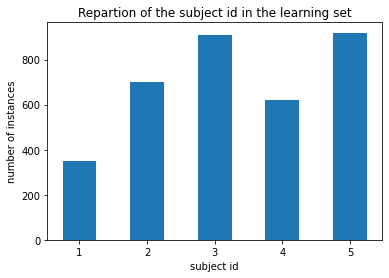
\includegraphics[scale = 0.5]{preprocessing/subjects_repartition.png}
\caption{Repartition of the different subject ID's in the learning set.}
\label{subject_repartition}
\end{figure}

\paragraph{}We observed that the learning set seems to be balanced. The activity ID's are well distributed: they are each composed of 250 instances of the subjects in the training set. However, when looking at the subject ID's of the learning set, we observed that some subjects have been less used to perform measures. This can be observed on the figure \ref{subject_repartition}.
This can lead to overfit: all subjects have not the same behavior when perfoming an activity and the sensors measures are correlated to one subject. We tried to make the sample relative to sensors and did feature selection on them to handle this problem. It was then difficult to predict the activity of the input subjects because the samples were not anymore link to one subject. We did not really find others solutions.

\paragraph{}We observed that the learning set seems to be balanced. We can see on the figure at the top right that the activity ID's are well distributed: they are each composed of 250 instances of the subjects in the training set. However, when looking at the subject ID's of the learning set, we observed that some subjects have been less used to perform measures. This can be observed on the figure at the top right.
This can lead to overfit: all subjects have not the same behavior when performing an activity and the sensors measures are correlated to one subject.

\paragraph{}These observations and the fact that the dataset was really huge (3500 * 31 * 512 values), motivated us to perform features selection. We decided to perform feature selection using \texttt{SelectFromModel}\footnote{\url{https://scikit-learn.org/stable/modules/feature_selection.html}}. It is performing ranking based on one estimator and then remove the less ranked features recursively. We chose the \texttt{ExtraTreeClassifier}\footnote{\url{https://www.geeksforgeeks.org/ml-extra-tree-classifier-for-feature-selection/}} as estimator for this method. It is similar to a random tree classifier and only differ in the manner it is constructed which lead to the creation of multiple de-correlated decision trees. This seems us to be a good model to rank the features because we have seen in the theoretical course that decision trees are nice to discriminate features but are too much related to the dataset. It is why the way the Extremely Randomized Trees are constructed reduce the variance link to the dataset and thus reduce the chances of overfitting.
\paragraph{}The fact that the feature sizes were really huge (31 * 512 features per subject), motivated us to perform features selection. We decided to perform feature selection using \texttt{SelectFromModel}\footnote{\url{https://scikit-learn.org/stable/modules/feature_selection.html}}. It is perfoming ranking based on one estimator and then remove the less ranked features recursively. We chose the \texttt{ExtraTreeClassifier}\footnote{\url{https://www.geeksforgeeks.org/ml-extra-tree-classifier-for-feature-selection/}} as estimator for this method. It is similiar to a random tree classifier and only differ in the manner it is constructed which lead to the creation of multiple de-correlated decision trees. This seems us to be a good model to rank the features because we have seen in the theoritical course that decision trees are nice to discriminate features but are too much related to the dataset. It is why the way the Extremely Randomized Trees are constructed reduce the variance link to the dataset and thus reduce the chances of overfitting.

\subsection{Implementation}

The implementation of this part can be found in the \texttt{preprocessing.ipynb} notebook or in the \texttt{preprocessing.py} python script. We have performed some tests measuring the scores and it is a bit increasing the scores of our models.

%%%%%%%%%%%%%%%%%%%%%%%%%%%%%%%%%%%%%%%%%%

\section{Studied models}

%%%%%%%%%%%%%%%%%%%%%%%%%%%%%%%%%%%%%%%%%%

\subsection{K-nearest neighbors}
\paragraph{}First, we decided to use the K-nearest neighbors method because it was the one provided by the pedagogical team with the assignment. Yet, the reasons that made us trying multiple versions of this technique are the facts that it is easy to interpret and to use.

\subsubsection{1-NN} \label{subsubsec:1NN}
\paragraph{}Our first submission was the one provided with assignment\footnote{File \texttt{example\_submission.csv}.} that was generated with the 1-nearest neighbor model\footnote{Files \texttt{toy\_script.py} or \texttt{knn\_basic\_1.py}.}.\\
This submission yields a score of 0.52 on Kaggle.

\subsubsection{25-NN} \label{subsubsec:25NN}
\paragraph{}Based on \ref{subsubsec:1NN}, we decided to increase the value of K of the K-nearest neighbors method to 25. The motivation behind the choice of this value for K was theoretical. Since the dataset is huge and can contain errors in the measured values, we though that increasing the value of K would increase the precision of the model because each prediction will not depend on a single neighbor that could have been misclassified.\\
This technique is implemented in the file \texttt{knn\_basic\_25.py}. This submission yields a score of 0.54 on Kaggle.

\subsubsection{55-NN and 49-NN} \label{subsubsec:55-49-NN}
\paragraph{}We decided to keep using the K-NN method to study how well it could perform on the assignment. We decided to study the accuracy of the KNN technique by using a 10-fold cross validation technique with the negative log loss function as a scoring measure. We obtained the following graph of accuracies depending on the value of K:
\begin{figure}[H]
\center
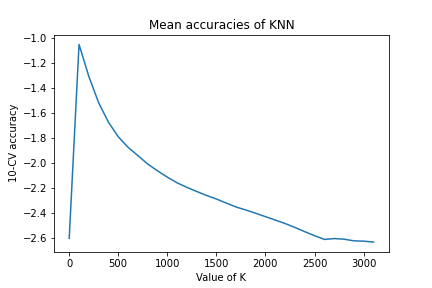
\includegraphics[scale=0.3]{knn/log_loss.png}
\caption{10-CV accuracy of KNN depending on value of K}
\end{figure}
We could see that there is a peak. By using a divide and conquer technique, we found that the peak was obtained for values of K around 50. Thus, we decided to study the accuracy in a small range of K values around $K=50$. We obtained the following graph:
\begin{figure}[H]
\center
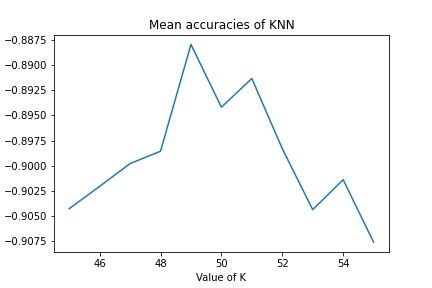
\includegraphics[scale=0.4]{knn/log_loss_focused.png}
\caption{10-CV accuracy of KNN depending on value of K}
\label{fig:knn_log_loss_focused}
\end{figure}
\paragraph{}Based on the divide and conquer approach performed, we decided to use 55 neighbors. The choice of this value was motivated by the fact that we observed a peak around this value.\\
This submission yields a score of 0.53142 on Kaggle and the implementation of it is inside the file \texttt{knn\_basic\_55.py}.
\paragraph{}Then, based on the graph of figure \ref{fig:knn_log_loss_focused}, we decided to use 49 neighbors. The choice of this value was motivated by the fact that it yields the highest score on the learning set by using a 10-fold cross validation strategy with the negative log loss function as a scoring measure.\\
This submission yields a score of 0.52571 on Kaggle which is less than the one for 55-NN. Yet, we expected a higher score based on the graph of figure \ref{fig:knn_log_loss_focused}. The implementation is available inside the file \texttt{knn\_basic\_49.py}.
\paragraph{}Based on the two previous results, we came to the conclusion that using "vanilla" K-nearest neighbors was not sufficient. Thus, we decided to find new techniques explained in the following sections.

\subsubsection{Multiple K-nearest neighbors models} \label{subsubsec:knnMultiple}
\paragraph{}We took a look back at the slides provided with the assignment and we focused on the features (sensors) of the datasets. We noticed that the features are not in the same units. Thus, we thought about using multiple 1-nearest neighbor models with one 1-NN model per feature. This idea was motivated by the fact that we though we would obtained a better accuracy by using one 1-NN per feature because measurements in different units would not be mixed.\\
We implemented this approach in the file \texttt{knn\_splitted\_1.py}. This yields a score of 0.52 on Kaggle which is the same as the toy script provided with the assignment.

\subsubsection{Mutiple K-nearest neighbors models and samples modification} \label{subsubsec:knnMultipleModif}
\paragraph{}After the disappointing result obtained in \ref{subsubsec:knnMultiple}, we decided to take a better a look at the datasets. We noticed that some samples were vectors full of -999999.99. We though that these measurements would badly influenced the models. Thus, we decided to replace each sample that was a vector full of -999999.99 by a vector full of 0.\\
We implemented this approach in the file \texttt{knn\_splitted\_1\_filtered.py} and the score obtained on Kaggle was 0.53142.

\subsubsection{Conclusion on K-nearest neighbors}
\paragraph{}After all the different tries perform using K-nearest neighbors models, we came to the conclusion that "vanilla" K-NN were not sufficient for this project.\\
The codes for the different plots are available inside the Jupyter notebooks \texttt{knn\_basic.ipynb} and \texttt{knn\_splitted.ipynb}.

%%%%%%%%%%%%%%%%%%%%%%%%%%%%%%%%%%%%%%%%%%

\subsection{Decision trees}\label{subsec:dt}
\paragraph{}Secondly, we decided to use the decision tree method because its interpretability is very easy and the effect of the parameters is easy to understand.

\subsubsection{Decision tree with min\_sample\_split=2} \label{subsubsec:dt2}
\paragraph{}First, we try a very simple decision tree with the parameter \texttt{min\_sample\_split} set to 2. We decided to choose this value for that parameter because we wanted to have a first result for the decision tree on which we could based our further study of the approach.\\
This model has been implemented in the file \texttt{dt\_basic\_2.py}. It has an accuracy of 0.8074285714285715 measured with a 10-fold cross validation strategy and provided a score of 0.38571 on Kaggle.

\subsubsection{Decision tree with post-pruning} \label{subsubsec:dtPruning}
\paragraph{}We decided to study the accuracy of the decision tree depending on the value of the \texttt{min\_sample\_split} parameter. In order to do, we decided to study the accuracy for values of the parameter ranging from 2 to 15500. We obtained the following graph:
\begin{figure}[H]
\centering
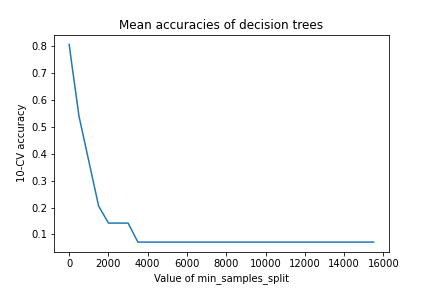
\includegraphics[scale=0.4]{dt/dt_basic_accuracies_1.png}
\caption{Accuracy of decision tree depending on value of parameter}
\label{fig:dt_acc_1}
\end{figure}
Based on figure \ref{fig:dt_acc_1}, we can see that the value of the parameter, that results in the highest accuracy, is smaller than 2000. Thus, we decided to study the accuracy of the model for values of the parameter between 2 and 2000. We obtained the following graph:
\begin{figure}[H]
\centering
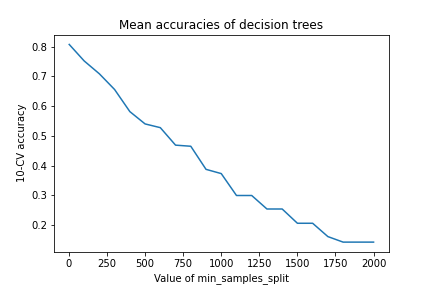
\includegraphics[scale=0.4]{dt/dt_basic_accuracies_2.png}
\caption{Accuracy of decision tree depending on value of parameter}
\end{figure}
We continue this approach and study the accuracy of the model for values of the parameter [2,200], [2,25], and [2,5]. We obtained the following graphs:
\begin{table}[H]
\centering
\begin{tabular}{lll}
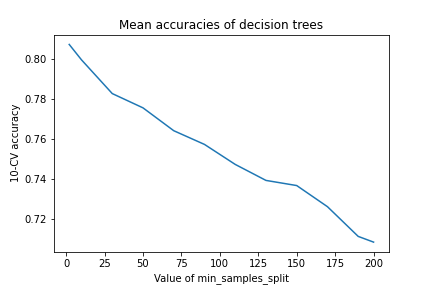
\includegraphics[scale=0.35]{dt/dt_basic_accuracies_3.png} & 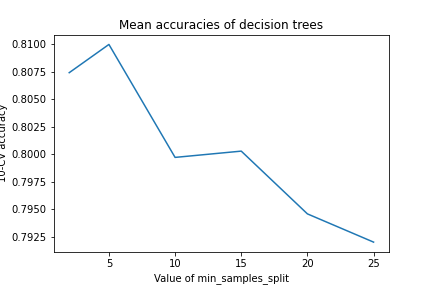
\includegraphics[scale=0.35]{dt/dt_basic_accuracies_4.png} & 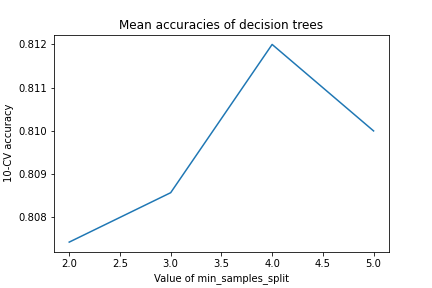
\includegraphics[scale=0.35]{dt/dt_basic_accuracies_5.png}
\end{tabular}
\end{table}
It turns out that using that using a small value for the parameter \texttt{min\_sample\_split} provides a higher accuracy using a 10-fold cross validation strategy. Yet, we might overfit on unseen data. Thus, we decided to study the overfitting. We based ourselves on the approach presented in the documentation of scikit-learn\footnote{https://scikit-learn.org/stable/auto\_examples/tree/plot\_cost\_complexity\_pruning.html\#}.
\paragraph{}We split the learning sample in 2 using proportions 75\% and 25\% where the 75\% will be our new learning set and the 25\% will be our new test set. Then, we computed the path during the minimal cost-complexity pruning and we got the alphas for the sub-trees. Afterwards, we build a tree with the different values of alphas obtained in the previous step\footnote{We actually build only a fifth because there was too much possible alphas.}. Finally, we computed the score of the LS and the TS on the different tress and plotted it. We obtained the following graphs:
\begin{table}[H]
\centering
\begin{tabular}{ll}
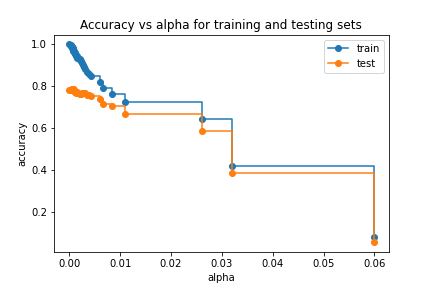
\includegraphics[scale=0.35]{dt/dt_pruning_study.png} & 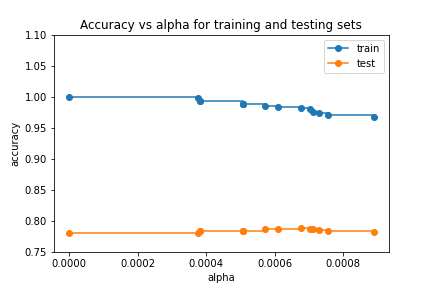
\includegraphics[scale=0.35]{dt/dt_pruning_study_zoomed.png}
\end{tabular}
\end{table}
Based on the obtained data, we found out that the value of alpha that provides the highest score on the test set was 0.0006772486772486773.\\
So, for our next model, we built a decision tree with this particular value of alpha for pruning. This particular model provided an accuracy of 0.8025714285714285 using a 10-fold cross validation approach and a score of 0.40285 on Kaggle, which is small improvement compared to the score 0.38571 obtained without pruning.\\
The analysis performed for this subsection is available in the Jupyter notebook \texttt{dt.ipnyb} and the implementation of the model in the file \texttt{dt\_pruned.py}.

\subsubsection{Decision tree with filtered data} \label{subsubsec:dtFiltered}
\paragraph{}As explained in section \ref{sec:data-pre-process}, the data provided is not ideal. Thus, we decided to try a decision tree with pre-processed data.\\
This model is implemented in the file \texttt{dt\_filtered.py}. This particular model provided an accuracy of 0.7928571428571429 using a 10-fold cross validation approach\footnote{Available in the Jupyter notebook \texttt{dt\_filtered.ipynb}.} and a score of 0.43428 on Kaggle. This is an improvement compared to the 0.40285 obtained with pruning.

\subsubsection{Conclusion on decision trees}
\textcolor{red}{TO BE ADDED}

%%%%%%%%%%%%%%%%%%%%%%%%%%%%%%%%%%%%%%%%%%

\subsection{Random forests}
\paragraph{}Next, we decided to use random forests because they should provide better accuracies than decision trees. Yet, their interpretability is still easy.

\subsubsection{Random forest with 40 trees} \label{subsubsec:rf40Trees}
\paragraph{}First, we decided to try a few forests and measuring their accuracies using a 10-fold cross validation approach. We obtained the following results:
\begin{table}[H]
\centering
\begin{tabular}{|l|l|l|l|}
\hline
\multicolumn{1}{|c|}{\textbf{\#}} & \multicolumn{1}{c|}{\textbf{Number of trees}} & \multicolumn{1}{c|}{\textbf{min\_sample\_split}} & \multicolumn{1}{c|}{\textbf{10-CV accuracy}} \\ \hline
1 & 10 & 200 & 0.7354285714285714 \\ \hline
2 & 50 & 200 & 0.7702857142857142 \\ \hline
3 & 50 & 100 & 0.8608571428571429 \\ \hline
4 & 100 & 50 & 0.9062857142857143 \\ \hline
\end{tabular}
\caption{10-CV accuracy of different random forests}
\label{tab:rf-acc}
\end{table}
Based on table \ref{tab:rf-acc}, the first conclusion we draw was that increasing the number of trees and diminishing the value of \texttt{min\_sample\_split} increases the accuracy measured with a 10-fold cross validation approach.
\paragraph{}Then, we decided to study the accuracy of the forest based on the number of trees with a fixed value for \texttt{min\_sample\_split} (arbitrarily set to 25). We obtained the following graph:
\begin{figure}[H]
\centering
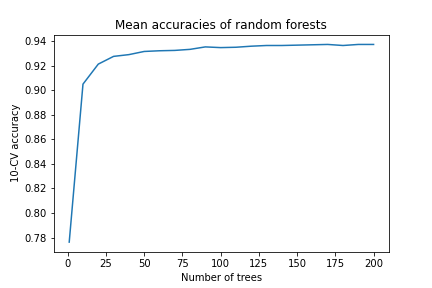
\includegraphics[scale=0.4]{rf/rf_basic_accuracies.png}
\caption{Accuracy of random forests depending on number of trees}
\label{fig:rf-acc-1}
\end{figure}
Based on figure \ref{fig:rf-acc-1}, we can see that, for a number of trees greater or equal to 30, we reach a plateau. Now, we will study the accuracy of random forests depending on the value of \texttt{min\_sample\_split} for a number of trees fixed to 40. We obtained the following graph:
\begin{figure}[H]
\centering
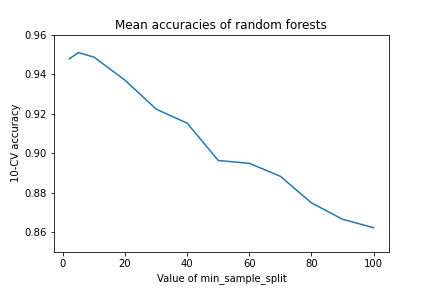
\includegraphics[scale=0.4]{rf/rf_40_accuracies.png}
\caption{Accuracy of random forests depending on \texttt{min\_sample\_split}}
\label{fig:rf-acc-2}
\end{figure}
As we can see on figure \ref{fig:rf-acc-2}, the smaller the value of \texttt{min\_sample\_split}, the higher the accuracy using a 10-fold cross validation measure.
\paragraph{}Based on a what we have observed, we decided to try a random forest composed of 40 trees with \texttt{min\_sample\_split} set to 25.\\
This model is implemented in the file \texttt{rf\_40\_25.py} and the analysis performed is available in the Jupyter notebook \texttt{random\_forest.ipynb}.\\
This model provided an accuracy of 0.9288571428571428 using a 10-fold cross validation strategy and a score of 0.52 on Kaggle. This score on Kaggle is the same as the one obtained for 1-NN. Yet, this is an improvement compared to the scores obtained for the decisions tree in the part \ref{subsec:dt} of this report. This is what was expected because random forests use multiple trees.

\subsubsection{Random forest with filtered data} \label{subsubsec:rfFiltered}
\paragraph{}As explained in section \ref{sec:data-pre-process}, the data provided is not ideal. Thus, we decided to try a random forest with pre-processed data. We kept the same values for the number of trees and \texttt{min\_sample\_split}.\\
This model is implemented in the file \texttt{rf\_filtered.py}. This particular model provides an accuracy of 0.9074285714285713 using a 10-fold cross validation approach\footnote{Available in the Jupyter notebook \texttt{random\_forest\_filtered.ipynb}.} and a score of 0.48285 on Kaggle. This is less than what we obtained for a random forest without filtering the data.

\subsubsection{Conclusion on random forests}
\paragraph{}\textcolor{red}{TO BE ADDED!}

%%%%%%%%%%%%%%%%%%%%%%%%%%%%%%%%%%%%%%%%%%

\subsection{Support vector machines}
\paragraph{}For completeness, we wanted to try support vector machines.

\subsubsection{Support vector classification} \label{subsubsec:svc}
\paragraph{}This approach is based on the model SVC of scikit-learn\footnote{sklearn.svm.SVC.}. We decided to study the accuracy of this model by splitting the learning set based on the ids of the 5 subjects and by using feature selection.\\
For our first study, we decided to consider a wide range for the value of the regularization parameter\footnote{Denoted C in scikit-learn.}. We choose the range [1.0, 1000.0] has a starting point and obtained the following graph of accuracies depending on the value of the parameter:
\begin{figure}[H]
\centering
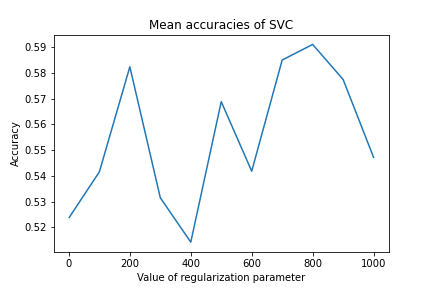
\includegraphics[scale=0.4]{svm/svm_svc_accuracies_1.png}
\caption{Accuracy of SVC depending on regularization parameter}
\end{figure}
As we can see on the previous plot, it seems there is not an obvious relation between the regularization and the accuracy of the model. Thus, we decided to study the accuracy of the model for values of the regularization in the range [1.0, 100.0]. We obtained the following graph:
\begin{figure}[H]
\centering
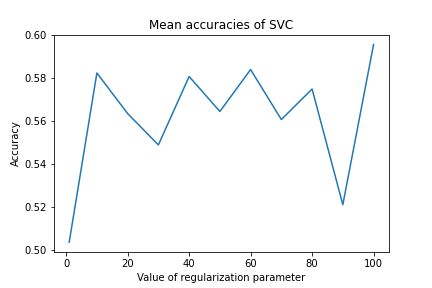
\includegraphics[scale=0.4]{svm/svm_svc_accuracies_2.png}
\caption{Accuracy of SVC depending on regularization parameter}
\end{figure}
Once again, it seems there is no obvious relation between the regularization and the accuracy. Yet, the values for the previous graphs were obtained as averages on 10 tries. We decided to increase the number of tries to 20. We obtained the following graph:
\begin{figure}[H]
\centering
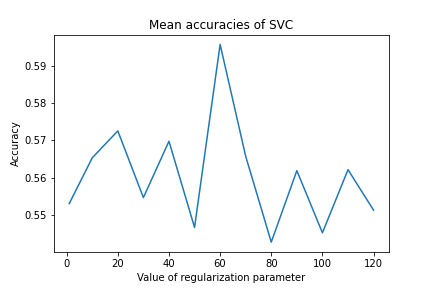
\includegraphics[scale=0.4]{svm/svm_svc_accuracies_4.png}
\caption{Accuracy of SVC depending on regularization parameter}
\end{figure}
The peak observed on the graph is for a value of the regularization parameter of 60. Thus, we decided to use a SVM (specifically \texttt{sklearn.svm.SVC}) with a value of 60 as the regularization parameter. This models has an accuracy 0.5956468368018641 locally obtained by splitting the learning set based on the ids of the 5 subjects and by using feature selection\footnote{The accuracies are averages over 20 tries.}. This model gives a score of 0.49428 on Kaggle.\\
The study performed for this model is available in the Jupyter notebook \texttt{svc-feature-extract\\ion.ipynb} and the implementation of the model in the file \texttt{svc-reg-60.py}.

\subsubsection{Support vector classification - $\nu$-SVC} \label{subsubsec:nusvc}
\paragraph{}This approach is based on the model $\nu$-SVC of scikit-learn\footnote{sklearn.svm.NuSVC}. As always, we decided to study the accuracy of the model depending on the value of the parameter $\nu$. To study the accuracy, we split the learning set based on the ids of the 5 subjects and by calculating average accuracies over multiples splits. We used feature selection to reduce the size of the learning set.\\
We study the accuracy of the model for values of $\nu$ in [0.1, 0.6]. We obtained the following graph:
\begin{figure}[H]
\centering
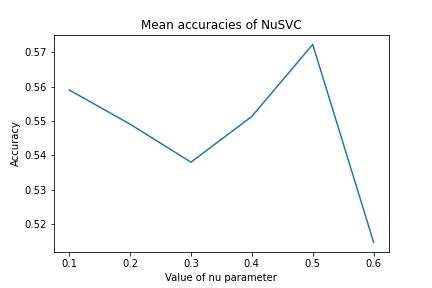
\includegraphics[scale=0.4]{nusvm/svm_nu_svc_accuracies_1.png}
\caption{Accuracy of $\nu$-SVC depending on value of $\nu$}
\end{figure}
The peak observed on the graph is for a value of $\nu$ of 0.5. Thus, we decided to use a $\nu$-SVC with $\nu = 0.5$. This model has an accuracy 0.5723277462764307 locally measured as explained before and a score on Kaggle of 0.56571.\\
The code for the generation of the graph is available in the Jupyter notebook \texttt{nusvc-feature-\\extraction.ipynb} and the implementation of the model in the file \texttt{nusvc.py}.

%%%%%%%%%%%%%%%%%%%%%%%%%%%%%%%%%%%%%%%%%%

\section{Summary table}
\paragraph{}The following table summaries the techniques we have tried and the scores we have obtained on Kaggle.
\begin{table}[H]
\centering
\begin{tabular}{|l|l|l|}
\hline
\multicolumn{1}{|c|}{\textbf{Approach}}                     & \multicolumn{1}{c|}{\textbf{Report section}} & \multicolumn{1}{c|}{\textbf{Kaggle score}} \\ \hline
1-NN                                                        & \ref{subsubsec:1NN}                          & 0.52                                       \\ \hline
25-NN                                                       & \ref{subsubsec:25NN}                         & 0.54                                       \\ \hline
55-NN                                                       & \ref{subsubsec:55-49-NN}                     & 0.53142                                    \\ \hline
49-NN                                                       & \ref{subsubsec:55-49-NN}                     & 0.52571                                    \\ \hline
Multiple 1-NN                                               & \ref{subsubsec:knnMultiple}                  & 0.52                                       \\ \hline
Multiple 1-NN with filtered data                            & \ref{subsubsec:knnMultipleModif}             & 0.53142                                    \\ \hline
Decision tree - min\_sample\_split=2                        & \ref{subsubsec:dt2}                          & 0.38571                                    \\ \hline
Decision tree with pruning                                  & \ref{subsubsec:dtPruning}                    & 0.40285                                    \\ \hline
Decision tree with filtered data                            & \ref{subsubsec:dtFiltered}                   & 0.43428                                    \\ \hline
Random forest - 40 trees - min\_sample\_split=25            & \ref{subsubsec:rf40Trees}                    & 0.52                                       \\ \hline
Random forest - filtered data                               & \ref{subsubsec:rfFiltered}                   & 0.48285                                    \\ \hline
MLP - 1 inner layer - 500 neurons                           & TO BE ADDED                                  & 0.48285                                    \\ \hline
MLP - 1 inner layer - 100 neurons                           & TO BE ADDED                                  & 0.43428                                    \\ \hline
MLP - 1 inner layer - 100 neurons - feature extraction      & TO BE ADDED                                  & 0.22                                       \\ \hline
25-NN with feature extraction                               & TO BE ADDED                                  & 0.45714                                    \\ \hline
Random forest - 1000 trees with feature extraction          & TO BE ADDED                                  & 0.87428                                    \\ \hline
Logistic regression with feature extraction                 & TO BE ADDED                                  & 0.48285                                    \\ \hline
SVM with feature extraction                                 & TO BE ADDED                                  & 0.07142                                    \\ \hline
SGD with feature extraction                                 & TO BE ADDED                                  & 0.07142                                    \\ \hline
SVM with feature extraction                                 & \ref{subsubsec:svc}                          & 0.49428                                    \\ \hline
NuSVC with feature extraction                               & \ref{subsubsec:nusvc}                        & 0.56571                                    \\ \hline
Random forest - 1000 trees with improved feature extraction & TO BE ADDED                                  & 0.91142                                    \\ \hline
\end{tabular}
\caption{Approaches with respective Kaggle scores}
\end{table}

%%%%%%%%%%%%%%%%%%%%%%%%%%%%%%%%%%%%%%%%%%
\end{document}